\section{Wahrscheinlichkeitstheorie}

\begin{frame}{Wahrscheinlichkeitstheorie vs. Statistik}
    \begin{itemize}
        \item Die \textbf{Wahrscheinlichkeitstheorie} versucht, die Ungewissheit zu \textbf{modellieren}. Es können also Vorhersagen gemacht werden (z.B. Umfragen vor einer Wahl).
        \item Die \textbf{beschreibende} (deskriptive) \textbf{Statistik} versucht, die Beobachtungen zu \textbf{beschreiben}. Es können keine Vorhersagen gemacht werden. 
        (Bsp.: Kommentare zum Ausgang einer Wahl, wie hat eine Personengruppe gewählt, etc...)
    \end{itemize}
\end{frame}

%%%%%%%%%%%%%%%%%%%%%%%%%%%%%%%%%%%%%%%%%%%%%%%%%%%%%%%%%%%%
%%%%%%%%%%%%%%%%%%%%%%%%%%%%%%%%%%%%%%%%%%%%%%%%%%%%%%%%%%%%
\subsection{Ereignisse und Wahrscheinlichkeiten}

\begin{frame}{Einführung am Beispiel: Sechsseitiger Würfel}
  \begin{itemize}
  \item \textbf{Zufallsexperiment}: der Würfel wird geworfen
  \item \textbf{Ergebnis} ist Element des Ergebnisraums:
    \begin{gather*}
      \Omega=\left\{\dice1,\dice2,\dice3,\dice4,\dice5,\dice6\right\}
    \end{gather*}
  \item \textbf{Ereignis} ist Teilmenge des Ergebnisraums $\Omega$
    \begin{itemize}
    \item $A = \left\{\dice1\right\}=$ \glqq eine 1 würfeln\grqq 
    \item $B = \left\{\dice2,\dice3\right\}=$\glqq eine 2 oder eine 3 würfeln\grqq 
    \item $C = \left\{\dice2,\dice4,\dice6\right\}=$\grqq eine gerade Zahl würfeln\grqq
    \end{itemize} 
  \item Ereignisse mit nur einem Element nennt man auch Elementarereignis
    \begin{itemize}
    \item Elementarereignis entspricht Ergebnis
    \end{itemize}
  \end{itemize}
\end{frame}

\begin{frame}{Die Menge der Ereignisse}
  \begin{itemize}
  \item \textbf{Potenzmenge} von $\Omega$: alle möglichen Teilmengen
    \begin{itemize}
    \item Achtung: $\{X,Y\} = \{Y,X\}$
    \end{itemize}
    \begin{multline*}
      \ereignisraum = \Bigl\{\emptyset
      ,\left\{\dice1\right\}
      ,\left\{\dice2\right\}
      ,\left\{\dice3\right\}
      ,\left\{\dice4\right\}
      ,\left\{\dice5\right\}
      ,\left\{\dice6\right\}
      ,\left\{\dice1,\dice2\right\}
      ,\dots
      ,\left\{\dice1,\dice6\right\}
      ,\\\left\{\dice2,\dice3\right\}      
      ,\left\{\dice3,\dice4\right\}
      ,\dots
      ,\left\{\dice3,\dice6\right\}      
      ,\dots
      ,\left\{\dice5,\dice6\right\}
      ,\\\left\{\dice1,\dice2,\dice3\right\}      
      ,\dots
      ,\left\{\dice1,\dice3,\dice4\right\}      
      ,\dots
      ,\left\{\dice4,\dice5,\dice6\right\} 
      ,\\\left\{\dice1,\dice2,\dice3,\dice4\right\}
      ,\left\{\dice3,\dice4,\dice5,\dice6\right\} 
      ,\\\left\{\dice1,\dice2,\dice3,\dice4,\dice5\right\}
      ,\left\{\dice2,\dice3,\dice4,\dice5,\dice6\right\} 
      ,\Omega\Bigr\}
    \end{multline*}
    \item Insgesamt $2^6$ Elemente
  \end{itemize}
\end{frame}

\begin{frame}{Wahrscheinlichkeiten}
  Die Wahrscheinlichkeit $P$ auf dem Ereignisraum $\ereignisraum$ ordnet
  jedem Element $A\in \ereignisraum$ eine Zahl zu. Es gilt:
  \begin{itemize}
  \item $0 \le P(A) \le 1$
  \item $P(\Omega) = 1$
  \item $P(A\cup B) = P(A)+P(B)$ falls $A\cap B=\emptyset$
    \begin{itemize}
    \item $P(A\cup B)$, Wahrscheinlichkeit, dass $A$ oder $B$ eintritt
    \end{itemize}
    \pause
  \item Dies gilt auch für beliebige Vereinigungen, wenn die Mengen
    sich paarweise nicht schneiden
    \begin{gather*}
      P\left(\bigcup_i A_i\right) = \sum_i P(A_i)
    \end{gather*}
  \end{itemize}
\end{frame}

\begin{frame}{Beispiel: sechsseitiger Würfel}
  \begin{itemize}
  \item Der Würfel ist nicht gezinkt:
    \begin{gather*}
      P(\{\dice1\}) = P(\{\dice2\}) = P(\{\dice3\}) = P(\{\dice4\}) = P(\{\dice5\}) = P(\{\dice6\}) = \frac16
    \end{gather*}
  \item Für Teilmengen $A$ mit $m$ Elementen gilt $P(A)=m/6$
    \begin{gather*}
      P(\{\dice1,\dice4\}) = \frac26=\frac13,
      \qquad
      P(\{\dice1,\dice4,\dice5\}) = \frac36=\frac12
    \end{gather*}
  \end{itemize}
\end{frame}

\begin{frame}{Beispiel: zwei sechsseitige Würfel}
  \begin{itemize}
  \item Zufallsexperiment: zwei identische Würfel werden gleichzeitig geworfen.
    \begin{gather*}
      \Omega = \left\{
        \begin{bmatrix}
          \dice1\\\dice1
        \end{bmatrix}
        ,
        \begin{bmatrix}
          \dice1\\\dice2
        \end{bmatrix}
        ,\dots,
        \begin{bmatrix}
          \dice1\\\dice6
        \end{bmatrix}
        ,
        \begin{bmatrix}
          \dice2\\\dice1
        \end{bmatrix}
        ,\dots,
        \begin{bmatrix}
          \dice2\\\dice6
        \end{bmatrix}
        ,
        \begin{bmatrix}
          \dice3\\\dice1
        \end{bmatrix}
        ,\dots,
        \begin{bmatrix}
          \dice6\\\dice6
        \end{bmatrix}
        \right\}
      \end{gather*}
    \item<3-> Bei identischen Würfeln kann die Reihenfolge nicht
      beobachtet werden, also nicht die Ereignisse
      \begin{gather*}
        \left\{\begin{bmatrix}
          \dice1\\\dice2
        \end{bmatrix}\right\}
        \quad\text{und}\quad
        \left\{\begin{bmatrix}
          \dice2\\\dice1
        \end{bmatrix}\right\}
      \quad\text{aber die Vereinigung}\quad
        \left\{\begin{bmatrix}
          \dice1\\\dice2
        \end{bmatrix}
        ,\begin{bmatrix}
          \dice2\\\dice1
        \end{bmatrix}\right\}
    \end{gather*}
  \item<3-> Wir definieren also den Ereignisraum
    \begin{gather*}
      \hspace*{-1em}
      \ereignisraum = \left\{\!
        \left\{\!
          \begin{bmatrix}
            \dice1\\\dice1
          \end{bmatrix}
          \!\right\}\!,\!
        \left\{\!
          \begin{bmatrix}
            \dice1\\\dice2
          \end{bmatrix}
          \!\!,\!\!
          \begin{bmatrix}
            \dice2\\\dice1
          \end{bmatrix}
          \!\right\}\!,\!
        \left\{\!
          \begin{bmatrix}
            \dice1\\\dice3
          \end{bmatrix}
          \!\!,\!\!
          \begin{bmatrix}
            \dice3\\\dice1
          \end{bmatrix}
          \!\right\}
        ,\dots,
        \left\{\!
          \begin{bmatrix}
            \dice2\\\dice2
          \end{bmatrix}
          \!\right\}
        \!,\!
        \left\{
          \begin{bmatrix}
            \dice2\\\dice3
          \end{bmatrix}
          \!\!,\!\!
          \begin{bmatrix}
            \dice3\\\dice2
          \end{bmatrix}
          \!\right\},\dots        
        \!\right\}
    \end{gather*}
    
  \end{itemize}
  \only<2>{
    \begin{Denkpause}
      Sind alle Ergebnisse beobachtbar?
    \end{Denkpause}
  }
\end{frame}

\begin{frame}{Ereignisraum und $\sigma$-Algebra}
  Ist $\ereignisraum$ nicht die Potenzmenge von $\Omega$, sondern eine
  andere Menge von Teilmengen, dann fordern wir folgende
  Eigenschaften:
  \begin{enumerate}
  \item $\Omega\in\ereignisraum$
  \item Falls $A\in\ereignisraum$, dann ist das Komplement $A^c\in\ereignisraum$.
  \item Falls $A_i\in\ereignisraum$ für $i=1,2,\dots$, dann ist
    \begin{gather*}
      \bigcup_{i} A_i\in\ereignisraum
    \end{gather*}
  \end{enumerate}
  Eine Menge von Teilmengen von $\Omega$ mit diesen Eigenschaften
  nennt man eine $\sigma$-Algebra über $\Omega$.

  \pause

  Auf einer $\sigma$-Algebra $\ereignisraum$ kann eine
  Wahrscheinlichkeit $P$ definiert werden.
\end{frame}

\begin{frame}{Beispiel: Konzentrationen}
  \begin{itemize}
  \item Ergebnis eines Zufallsexperiments: pH-Wert
    \begin{itemize}
    \item $\Omega = (0,14]$ (halboffen aus praktischen Gründen)
    \item Die Potenzmenge der reellen Zahlen ist ein mathematisches Monster
      \begin{itemize}
      \item Ungeeignet für die Definition der Wahrscheinlichkeit
      \end{itemize}
    \end{itemize}
    \pause
  \item Sie haben ein billiges pH-Meter, das nur ganzzahlig ausgibt
    \begin{itemize}
    \item Die \glqq{}Atome\grqq{} der passenden $\sigma$-Algebra sind die Mengen
      \begin{gather*}
        \bigl\{ x\in(0,14]\big| i-1<x\le i\bigr\},\quad i=1,\dots,14
      \end{gather*}
    \item Alle weiteren Teilmengen, inklusive $\Omega$ entstehen
      durch Vereinigungen
    \item Die $\sigma$-Algebra bildet mögliches Wissen über die Zufallsergebnisse ab
    \end{itemize}
    \pause
  \item Die sogenannte Borelsche $\sigma$-Algebra bildet den
    Informationsgehalt der reellen Zahlen ab
  \end{itemize}
\end{frame}

\begin{Aufgabe}
  Was wäre die $\sigma$-Algebra $\ereignisraum $ bei einem doppelten Münzwurf, falls
  \begin{enumerate}
  \item zwei Münzen gleichzeitig geworfen werden?
  \item zwei Münzen nacheiander geworfen werden?
  \end{enumerate}
\end{Aufgabe}

\begin{frame}{Überlappende Ereignisse}
  \begin{gather*}
    A\cap B \neq \emptyset
  \end{gather*}
  \begin{itemize}
  \item Die beiden Ereignisse können gleichzeitig eintreten
  \item  Beispiel Würfel:
    \begin{align*}
      A&=\left\{\dice2,\dice4,\dice6\right\},
      \\B&=\left\{\dice1,\dice2,\dice3\right\},
      \\A\cap B&= \left\{\dice2\right\} \\
      P(A\cap B) &= \frac{1}{6}
    \end{align*}
  \end{itemize}
\end{frame}

\begin{frame}{Siebformel für überlappende Ereignisse}
    \begin{itemize}
        \item Für 2 Ereignisse $A$ und $B$ gilt im Allgemeinen:
        \begin{gather*}
            P(A\cup B) = P(A) +P(B)-P(A\cap B)    
        \end{gather*}
        \item  Beispiel Würfel:
        \begin{gather*}
          A=\left\{\dice2,\dice4,\dice6\right\},
          \ B=\left\{\dice3,\dice4,\dice5,\dice6\right\},
          \ A\cap B= \left\{\dice4,\dice6\right\} \\
            \Rightarrow P(A\cap B) = \frac{2}{6}
        \end{gather*}
        \item also gilt 
        \begin{gather*}
            P(A\cup B)= \frac{3}{6} + \frac{4}{6} - \frac{2}{6} = \frac{5}{6}
        \end{gather*}
    \end{itemize}
\end{frame}

\begin{frame}{Siebformel für überlappende Ereignisse}
  Für $n$ Ereignisse gilt allgemein:
  \begin{multline*}
    P\left(\bigcup_iA_i\right)
    =\sum_iP(A_i)-\sum_{i<j}P(A_i\cap A_j) \\
    + \sum_{i<j<k}P(A_i\cap A_j \cap A_k) - \dots
  \end{multline*}

  \begin{itemize}
  \item Zunächst subtrahiert man von der Summe alle Schnitte, da diese
    doppelt gezählt wurden
  \item Dabei hat man aber die Schnitte dreier Ereignisse zweimal
    subtrahiert, deswegen addiert man sie wieder
  \item Nun hat man denselben Fehler mit Schnitten von vier Ereignissen gemacht
  \item ...
  \end{itemize}
\end{frame}

\begin{frame}{Eigenschaften der Wahrscheinlichkeit}
  \begin{itemize}
  \item Komplement $P(A^c) = 1-P(A)$, Wahrscheinlichkeit, dass $A$ nicht eintritt
  \item Unmögliches Ereignis $P(\emptyset)=0$
  \item wenn $A\subseteq B \Rightarrow P(A) \leq P(B)$
  \item $P(A\cup B)\leq P(A)+P(B)$
  \end{itemize}
\end{frame}

\begin{frame}{Bedingte Wahrscheinlichkeit}
    \begin{itemize}
        \item \textbf{Bedingte Wahrscheinlichkeit} bezeichnet die Wahrscheinlichkeit eines Ereignisses $A$ unter dem Wissen, dass Ereignis $B$ bereits eingetreten ist (geschrieben: $P(A|B)$
        \item Sie ist definiert als:
        \begin{gather*}
            P(A|B) = \frac{P(A\cap B)}{P(B)}
        \end{gather*}
        \item \textit{"Wie oft sind $A$ und $B$ aufgetreten, gemessen an der Häufigkeit von $B$ allein?}
    \end{itemize} 
    \includegraphics[width=0.8\textwidth]{fig/bedingte_Wahrscheinlichkeit.tikz}
\end{frame}

\begin{frame}{Vorsorgetests}
  \begin{itemize}
  \item Sie testen auf eine seltene, zunächst syptomlose Erkrankung
    \begin{itemize}
    \item Prävalenz 0.1\%
    \end{itemize}
  \item Die gesamte Bevölkerung wird getestet
    \begin{itemize}
    \item Sensitivität 99\%
    \item Spezifität 99\%
    \end{itemize}
  \item<3-> Bei Bevölkerung 1M sind 1000 erkrankt
    \begin{itemize}
    \item Positive Tests $1000\cdot 99\%=990$
    \end{itemize}
  \item<4-> Es sind $1M-1000= 999000$ gesund
    \begin{itemize}
    \item Positive Tests $999000\cdot 1\% = 9990$
    \end{itemize}
  \item<5-> Seien $T$ und $K$ die Ereignisse pos. Test und krank
    \begin{gather*}
      P(T) = \frac{10980}{1M},\quad
      P(T\cap K) = \frac{990}{1M},\quad
      P(K|T) = \frac{990}{10980} \approx 9\%
    \end{gather*}
    \item<5-> Die bedingte Wahrscheinlichkeit hängt von der Prävalenz ab
  \end{itemize}
  \begin{onlyenv}<2>
    \begin{Denkpause}
      Wie hoch ist bei einem positiven Testergebnis die
      Wahrscheinlichkeit, erkrankt zu sein?
    \end{Denkpause}
  \end{onlyenv}
\end{frame}

%%%%%%%%%%%%%%%%%%%%%%%%%%%%%%%%%%%%%%%%%%%%%%%%%%%%%
\begin{frame}
    \frametitle{Satz der totalen Wahrscheinlichkeit}
\label{totprob}
    \begin{center}
        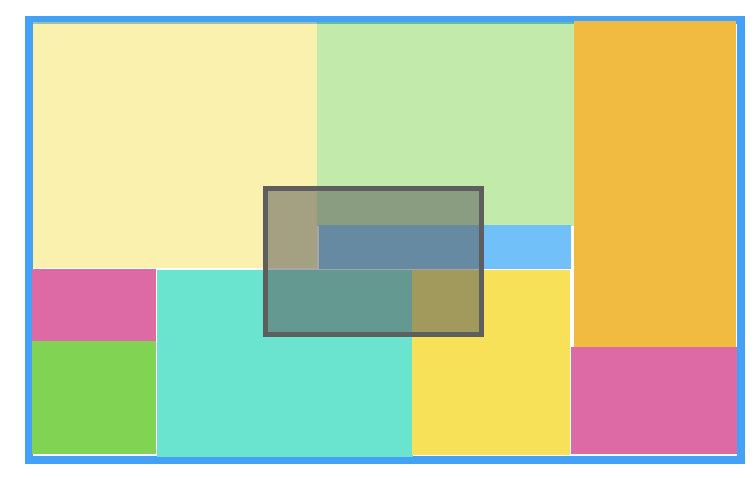
\includegraphics[width=.6\textwidth]{fig/prob03.png}
    \end{center}
    \begin{itemize}
    \item $A_i$ disjunkte Ereignisse, sodass $\cup_i A_i = \Omega$
    \item Dann gilt für ein Ereignis $B$:
      \begin{gather*}
        P(B) = \sum_i P(A_i)\frac{P(B\cap A_i)}{P(A_i)}
        \visible<2>{= \sum_i P(A_i)\,P(B|A_i)}
      \end{gather*}
    \end{itemize}
\end{frame}


%%%%%%%%%%%%%%%%%%%%%%%%%%%%%%%%%%%%%%%%%%%%%%%%%%%%%
\begin{frame}
    \frametitle{Bayes' Formel}

    \begin{itemize}
        \item Da $P(A\cap B) = P(B \cap A)$ können wir bei der Formel für die bedingte Wahrscheinlichkeit $A$ und $B$ vertauschen; daher gilt:
        $$
        P(A\cap B) = P(A|B)\,P(B) = P(B|A)\,P(A)
        $$  
        \item Daraus leiten wir die {\bf Bayessche Formel} her:
        $$
        P(A|B) = \frac{P(B|A)}{P(B)}\,P(A)
        $$
        \item $P(A)$ ist die {\em a priori} Wahrscheinlichkeit von $A$ (ohne vorheriges Wissen über andere Ereignisse!)
        \item $P(A|B)$ ist die {\em a posteriori} Wahrscheinlichkeit nach der Beobachtung von $B$
        \item Grundlage der Bayeschen Statistik
    \end{itemize}
\end{frame}

%%%%%%%%%%%%%%%%%%%%%%%%%%%%%%%%%%%%%%%%%%%%%%%%%%%%%%%%%%%%

\begin{frame}{Beispiel Vorsorgetest}
  \begin{itemize}
  \item Mit der Bayesschen Formel können wir die bedingte
    Wahrscheinlichkeit direkt ausrechnen:
    \begin{itemize}
    \item $P(K)$ Prävalenz
    \item $P(T|K)$ Sensitivität
    \item $1-P(T|K^c)$ Spezifität
    \end{itemize}
  \item Zu berechnen: $P(T)$
    \only<article>{unter Benutzung der totalen Wahrscheinlichkeit.}
    \begin{align*}
      P(T) &= P(T|K)P(K) + P(T|K^c)P(K^c) \\
      &= 0.99\times0.001 + 0.01\times 0.999 = 0.01098
    \end{align*}
  \item Einsetzen in Bayes' Formel ergibt
    \begin{align*}
      P(K|T) &= \frac{P(T|K)}{P(T)}P(K)\\
             &= \frac{0.99}{0.01098} \times  0.001 \approx 0.09016
    \end{align*}
  \end{itemize}
\end{frame}

%%%%%%%%%%%%%%%%%%%%%%%%%%%%%%%%%%%%%%%%%%%%%%%%%%%%%
\begin{frame}
  \frametitle{Bayes Formel und totale Wahrscheinlichkeit}

  Wir haben soeben folgende Eigenschaft benutzt, die sich aus der
  Kombination der Bayesschen Formel mit der totalen Wahrscheinlichkeit
  ergibt:
  \begin{itemize}
  \item $A_i$ disjunkte Ereignisse, sodass
    \begin{gather*}
      \bigcup_i A_i = \Omega
    \end{gather*}
  \item Dann gilt für ein Ereignis $B$:
    \begin{gather*}
      P(A_j|B) =  \frac{P(B|A_j)}{\sum_i P(B|A_i)P(A_i)}\,P(A_j)
    \end{gather*}
  \end{itemize}
\end{frame}

%%%%%%%%%%%%%%%%%%%%%%%%%%%%%%%%%%%%%%%%%%%%%%%%%%%%%
\begin{frame}
    \frametitle{Beispiel}

    \begin{itemize}
        \item Zwei Mitarbeiter einer Firma $M_1$, $M_2$ bearbeiten Anträge
        \item $M_1$ hat $P_1=40\%$ der Anträge bearbeitet, $M_2$ $P_2=60\%$
        \item $M_1$ hat eine Fehlerquote von 5\%, dh.\  $P(F|M_1)=0.05$
        \item $M_2$ hat eine Fehlerquote von 8\%, dh.\  $P(F|M_2)=0.08$
        \item Bei einem Antrag wurde eine fehlerhafte Bearbeitung festgestellt; was ist die Wahrscheinlichkeit, dass er von $M_1$ bearbeitet wurde?
        \item Lösung: wir suchen $P(M_1|F)$:
        \begin{eqnarray*}
        P(M_1|F) &=& \frac{P(F|M_1)}{P(F|M_1)P(M_1)+ P(F|M_2)P(M_2)}\,P(M_1) \\
        &=& \frac{0.05}{0.05\times 0.4 + 0.08\times 0.6}\times 0.4 = 29.4\%
        \end{eqnarray*}
    \end{itemize}
\end{frame}

%%%%%%%%%%%%%%%%%%%%%%%%%%%%%%%%%%%%%%%%%%%%%%%%%%%%%
\begin{frame}
    \frametitle{Unabhängige Ereignisse}

    \begin{itemize}
        \item Definition: zwei Ereignisse $A$ und $B$ sind {\bf unabhängig}, wenn gilt:
        $$
        P(A \cap B) = P(A)\cdot P(B)
        $$  
        \item Benutzt man die Bayes Formel folgt daraus: sind $A$ und $B$ unabhängig, dann gilt: $P(A|B) = P(A)$; das Wissen über $B$ verändert nicht die a posteriori Wahrscheinlichkeit von $A$
        \begin{itemize}
            \item Wahrscheinlichkeit, dass er regnet, gegeben, dass der Tag ein Montag ist: $P(Regen|Montag) = P(Regen)$
            \item Wahrscheinlichkeit, dass er regnet, gegeben, dass der Monat November ist: $P(Regen|November) \neq P(Regen)$ da Regen und November nicht unabhängig sind!
        \end{itemize}
    \end{itemize}
    

\end{frame}

%%%%%%%%%%%%%%%%%%%%%%%%%%%%%%%%%%%%%%%%%%%%%%%%%%%%%
\begin{frame}
  \frametitle{Unabhängige Ereignisse}
  
  \begin{itemize}
  \item Achtung: Unabhängigkeit und Disjunktheit sind nicht identisch!
  \item Disjunktheit von $A$ und $B$:
    \begin{gather*}
      P(A \cap B) =0
    \end{gather*}
  \item Unabhängigkeit von $A$ und $B$:
    \begin{gather*}
      P(A \cap B) =P(A)\,P(B)
    \end{gather*}
  \item \textbf{Vollständige} oder \textbf{gegenseitige} Unabhängigkeit bei mehreren Ereignissen $A_1,\ldots,A_k$: für jede Wahl von $k$ Ereignissen $A_{i_1},\ldots,A_{i_k}$ gilt:
    $$
    P(A_{i_1} \cap \ldots \cap A_{i_k}) = P(A_{i_1})\,P(A_{i_2})\ldots P(A_{i_k})
    $$
  \end{itemize}    
\end{frame}

%%%%%%%%%%%%%%%%%%%%%%%%%%%%%%%%%%%%%%%%%%%%%%%%%%%%%%%%%%%%
\begin{frame}{Beispiel: wiederholte Würfe eines Würfels}
  \begin{itemize}
  \item Ein sechsseitiger Würfel werde $5$ mal geworfen.
  \item In jedem Wurf ist die Wahrscheinlichkeit jeder Zahl 1/6
    \begin{itemize}
    \item ...unabhängig von allen vorherigen Würfen
    \end{itemize}
  \end{itemize}
  \begin{multline*}
    P\!\left(
      \begin{matrix}
        \dice6\\\dice6\\\dice6\\\dice6\\\dice6
      \end{matrix}
    \right)
    =
    P\!\left(
      \begin{matrix}
        \dice6\\ \\ \\ \\\phantom{\dice6}
      \end{matrix}
    \right)\times
    P\!\left(
      \begin{matrix}
        \\\dice6 \\ \\ \\\phantom{\dice6}
      \end{matrix}
    \right)\times
    P\!\left(
      \begin{matrix}
        \\ \\\dice6 \\ \\\phantom{\dice6}
      \end{matrix}
    \right)\times
    P\!\left(
      \begin{matrix}
        \\ \\ \\\dice6 \\\phantom{\dice6}
      \end{matrix}
    \right)\times
    P\!\left(
      \begin{matrix}
        \\ \\ \\ \\\dice6
      \end{matrix}
    \right)\\
    =\frac16\frac16\frac16\frac16\frac16 = \frac1{7776}
  \end{multline*}
\end{frame}


%%%%%%%%%%%%%%%%%%%%%%%%%%%%%%%%%%%%%%%%%%%%%%%%%%%%% 
\begin{frame}
  \frametitle{Abschlussfragen}
  
  \begin{enumerate}
  \item Was ist die Potenzmenge $\mathcal{S}$ beim Münzwurf (Kopf oder Zahl)?
  \item Müssen Sie Sensitivität oder Spezifität erhöhen, um den Test
    signifikant zu verbessern?
  \item Wieviele Anträge hätte $M_1$ bearbeiten müssen damit bei einem
    fehlerhaften Antrag eine 50/50 Chance besteht, dass er von $M_1$
    bearbeitet wurde?
  \end{enumerate}
\end{frame}
  


%%%%%%%%%%%%%%%%%%%%%%%%%%%%%%%%%%%%%%%%%%%%%%%%%%%%%
%%%%%%%%%%%%%%%%%%%%%%%%%%%%%%%%%%%%%%%%%%%%%%%%%%%%%
\subsection{Kombinatorik}
%%%%%%%%%%%%%%%%%%%%%%%%%%%%%%%%%%%%%%%%%%%%%%%%%%%%%

\begin{frame}{Zählen}
  \begin{itemize}
  \item Bei endlichen Ergebnismengen benötigt man die Anzahl aller
    Ergebnisse, um die Wahrscheinlichkeit zu berechnen
    \begin{gather*}
      P(A) = \frac{\#A}{\#\Omega}
    \end{gather*}
  \item Kombinatorik beschäftigt sich mit dem Zählen möglicher Ergebnisse
  \item Kombinatorik untersucht, wie viele verschiedene Anordnungen,
    Auswahlen oder Zuordnungen unter gegebenen Bedingungen möglich
    sind.
  \end{itemize}
\end{frame}

\begin{frame}{Permutationen}
  \begin{itemize}
  \item Permutationen von $n$ Objekten sind die möglichen Vertauschungen der Reihenfolge
  \item Ihre Anzahl ist
    \begin{gather*}
      n! = 1\cdot 2\cdot \ldots \cdot n      
    \end{gather*}
  \item Beispiel: $3!=6$
    \begin{gather*}
      (\dice1,\dice3,\dice5),(\dice1,\dice5,\dice3),\\
      (\dice3,\dice1,\dice5),(\dice3,\dice5,\dice1),\\
      (\dice5,\dice3,\dice1),(\dice1,\dice1,\dice3)\phantom{,}
    \end{gather*}
  \end{itemize}
\end{frame}



\begin{frame}
  \frametitle{Kombinationen}
  \begin{itemize}
  \item Auswahl von $k$ Objekten aus $n$
  \item Reihenfolge ist irrelevant
  \item Ihre Anzahl ist der Binomialkoeffizient
    \begin{gather*}
      \binom{n}{k} = \frac{n!}{k!(n-k)!}
    \end{gather*}
  \item Beispiel: Lotto 6 aus 49
    \begin{gather*}
      \frac{49!}{6!\,43!} = \frac{44\times 45\times \dots\times 49}{6!}
      = \frac{10068347520}{720} = 13983816
    \end{gather*}
  \end{itemize}
\end{frame}    

\begin{frame}
  \frametitle{Variationen}
  \begin{itemize}
  \item Auswahl von $k$ Objekten aus $n$
  \item Die Reihenfolge zählt
  \item Ihre Anzahl ist
    \begin{gather*}
      \binom{n}{k}k! = \frac{n!}{(n-k)!}
    \end{gather*}
  \item Beispiel: Alle Ketten von zwei der DNA-Basen Adenin, Cytosin, Guanin und Thymin
    \begin{gather*}
      A-C 
    \end{gather*}
  \end{itemize}

\end{frame}

\begin{frame}
  \frametitle{Variationen mit Wiederholungen}
  \begin{itemize}
  \item Auswahl von $k$ Objekten aus $n$
  \item Die Reihenfolge zählt
  \item Objekte dürfen mehrfach auftreten
  \item Ihre Anzahl ist
    \begin{gather*}
      n^k
    \end{gather*}
  \item Beispiel: Alle Ketten von zwei der DNA-Basen Adenin, Cytosin, Guanin und Thymin
    \begin{gather*}
      \begin{matrix}
        A-A& A-C& A-G& A-T\\
        C-A& C-C& C-G& C-T\\
        G-A& G-C& G-G& G-T\\
        T-A& T-C& T-G& T-T
      \end{matrix}
      \qquad 4^2=16
    \end{gather*}
  \end{itemize}
\end{frame}

\begin{frame}
  \frametitle{Kombinationen mit Wiederholungen}
  \begin{itemize}
  \item Auswahl von $k$ Objekten aus $n$
  \item Reihenfolge irrelevant
  \item Objekte dürfen mehrfach auftreten
  \item Ihre Anzahl ist
    \begin{gather*}
      \binom{n+k-1}{k}
    \end{gather*}
  \item Beispiel: eine Schachtel mit 2 Macaron aus den Sorten Cassis, Framboise und Myrtille
    \begin{gather*}
      \{C,C\}, \{C,F\},\{C,M\},\{F,F\},\{F,M\},\{M,M\}
      \qquad
      \binom{3+2-1}{2} = \binom{4}{2} = 6
    \end{gather*}
  \end{itemize}
\end{frame}

%%%%%%%%%%%%%%%%%%%%%%%%%%%%%%%%%%%%%%%%%%%%%%%%%%%%%%%%%%%%
\begin{Abschluss}
\item Wie viele DNA-Sequenzen der Länge 20 gibt es?
\item Wie viele verschiedene Reihenfolgen können fünf Gene haben?
\item Wie viele Möglichkeiten gibt es, drei Proben aus zehn auszuwählen?  
\item Was ist wahrscheinlicher:
  \begin{enumerate}
  \item bei 4 Würfen mit einen Würfel wird mindestens eine 6 geworfen;
  \item bei 24 Würfen mit 2 Würfeln wird mindestens eine Doppelsechs geworfen
  \end{enumerate}
\item Wieviele Möglichkeiten gibt es, eine Schachtel mit 3 Macarons
  der Sorten Cassis, Framboise, Myrtille und Pamplemousse zu füllen,
  wobei beliebig viele von allen, Myrtille aber maximal einmal, drin
  sein dürfen?
\end{Abschluss}


%%%%%%%%%%%%%%%%%%%%%%%%%%%%%%%%%%%%%%%%%%%%%%%%%%%%%%%%%%%%
%%%%%%%%%%%%%%%%%%%%%%%%%%%%%%%%%%%%%%%%%%%%%%%%%%%%%%%%%%%%

\subsection{Zufallsvariablen}
\begin{itemize}
\item Wir definieren jetzt die {\bf Wahrscheinlichkeit} $P_X$ der Zufallsvariablen $X$ 
  \begin{eqnarray*}
    &&P_X([a,b]) \equiv P(X \in [a,b]) ~~~\text{(stetige ZV)} \\ 
    &&P_X(k) \equiv P(X=k) ~~~\text{(diskrete ZV)}
  \end{eqnarray*}
\item Die Wahrscheinlichkeit $P_X$ ist also eine Abbildung
  $$
  P_X : \mathbb{R} \text{ oder } \mathbb{N} \longrightarrow [0,1]
  $$
\end{itemize}


%%%%%%%%%%%%%%%%%%%%%%%%%%%%%%%%%%%%%%%%%%%%%%%%%%%%%
\begin{frame}
    \frametitle{Zufallsvariablen und Wahrscheinlichkeit}

    \centerline{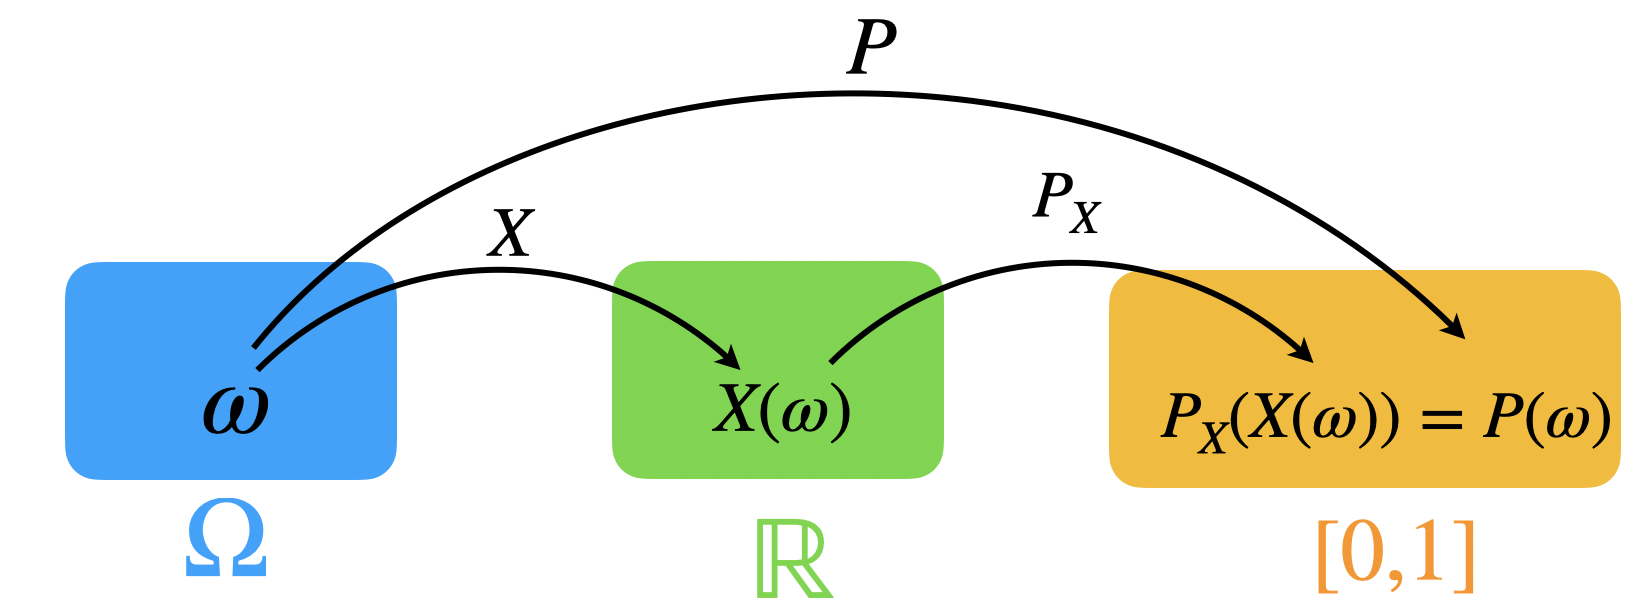
\includegraphics[width=.9\textwidth]{fig/prob09.png}}
\end{frame}

%%%%%%%%%%%%%%%%%%%%%%%%%%%%%%%%%%%%%%%%%%%%%%%%%%%%%
\begin{frame}
    \frametitle{Beispiel beim Münzspiel}


 \textbf{Ausgangssituation:}
\begin{itemize}
\item 3 Münzwürfe: $\Omega = {ZZZ, KZZ, ZKZ, ZZK, KKZ, KZK, ZKK, KKK}$
\item Jedes Ergebnis hat Wahrscheinlichkeit $(1/2)^3 = 1/8$
\end{itemize}
\vspace{0.5cm}
\textbf{Zufallsvariable} $X = $ "Anzahl der Zahlen"

\end{frame}

%%%%%%%%%%%%%%%%%%%%%%%%%%%%%%%%%%%%%%%%%%%%%%%%%%%%%
\begin{frame}
    \frametitle{Beispiel beim Münzspiel}

\textbf{Schritt 1:} Welche Werte kann $X$ annehmen?
\begin{itemize}
\item $X$ kann 0, 1, 2 oder 3 sein
\end{itemize}
\vspace{0.5cm}
\textbf{Schritt 2:} Für jeden Wert - welche Elementarereignisse führen dazu?

\vspace{0.5em}
\begin{tabular}{llll}
$X = 0$ & $\text{nur } KKK$ &$\Rightarrow$ & $P_X(0) = P(X = 0) = 1/8$\\
$X = 1$ & $KKZ, KZK, ZKK$ & $\Rightarrow$ & $P_X(1)=P(X = 1) = 3/8$\\
$X = 2$ & $KZZ, ZKZ, ZZK$ &$\Rightarrow$ & $P_X(2)=P(X = 2) = 3/8$\\
$X = 3$ & $\text{nur } ZZZ$ & $\Rightarrow$ & $P_X(3)=P(X = 3) = 1/8$
\end{tabular}
\end{frame}


%%%%%%%%%%%%%%%%%%%%%%%%%%%%%%%%%%%%%%%%%%%%%%%%%%%%%
\begin{frame}
    \frametitle{Diskrete Zufallsvariablen}

    \begin{itemize}
        \item Zufallsvariable: $X$ ; mögliche Realisationen: $x_i$
        \item Für diskrete Zufallsvariablen betrachten wir die {\bf Wahrscheinlichkeitsverteilung} 
        $$
        p_i = P(X = x_i)~~~~x_i = \text{abzählbare Realisationen}
        $$
        \item Es gilt
        $$
        \sum_i P(X=x_i) = 1
        $$  
        \item Die {\bf Verteilungsfunktion} ist hier:
        $$
        F_X(x) = P(X \le x) = \sum_{i: x_i \le x} P(X=x_i)
        $$
    \end{itemize}

\end{frame}

%%%%%%%%%%%%%%%%%%%%%%%%%%%%%%%%%%%%%%%%%%%%%%%%%%%%%
\begin{frame}
    \frametitle{Diskrete Zufallsvariablen}

    
    \begin{center}
        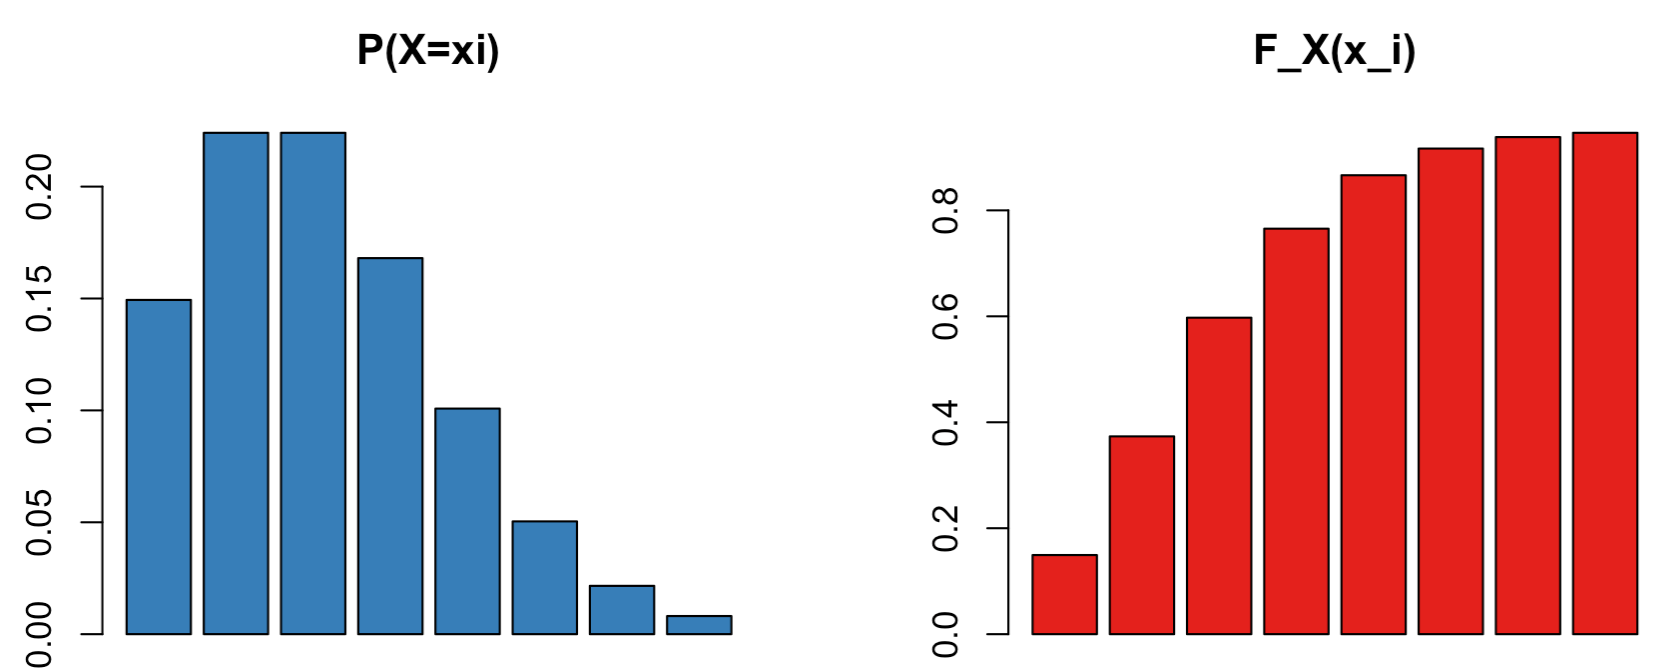
\includegraphics[width=.9\textwidth]{fig/prob04.png}
    \end{center}
    

\end{frame}




%%%%%%%%%%%%%%%%%%%%%%%%%%%%%%%%%%%%%%%%%%%%%%%%%%%%%
\begin{frame}
    \frametitle{Stetige Zufallsvariablen}

    \begin{itemize}
        \item Bei stetigen Zufallsvariablen ("Körpergröße; Regenmenge in einem Jahr; ...") gilt
        $
        P(X = x) =0
        $
        \item Anders ausgedrückt: Die Wahrscheinlichkeit, eine Person zu finden, die {\bf GENAU} 1,6 Meter groß ist ist Null \dots
        \item Wir betrachten stattdessen  die {\bf Wahrscheinlichkeitsdichte} $f(x): \mathbb{R} \to \mathbb{R}$ mit folgenden Eigenschaften:
    \end{itemize}
        \begin{enumerate}
            \item $P_X([a,b]) = P(X\in [a,b])= \int_{a}^{b} f(x)\,dx$ 
            \item $\int_{-\infty}^{\infty} f(x)\,dx = 1$
            \item $F_X(a) = P(X \le a) = \int_{-\infty}^{a} f(x)\,dx$
        \end{enumerate}
    

\end{frame}

%%%%%%%%%%%%%%%%%%%%%%%%%%%%%%%%%%%%%%%%%%%%%%%%%%%%%
\begin{frame}
    \frametitle{Stetige Zufallsvariablen}

    
    \begin{center}
        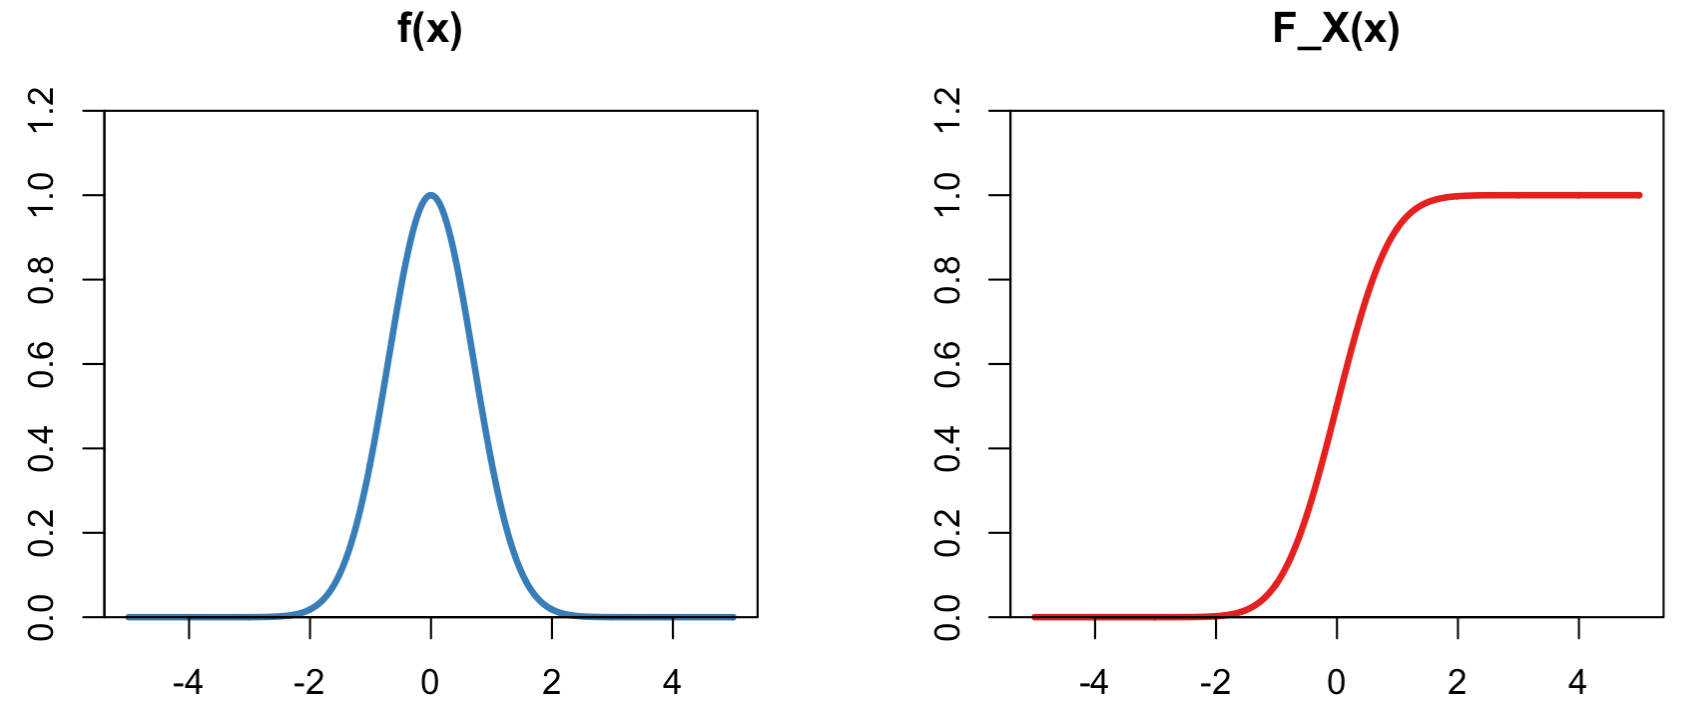
\includegraphics[width=.9\textwidth]{fig/prob05.png}
    \end{center}
    

\end{frame}




%%%%%%%%%%%%%%%%%%%%%%%%%%%%%%%%%%%%%%%%%%%%%%%%%%%%%
\begin{frame}
    \frametitle{Erwartungswert}

    Beispiel: Spiel mit gezinkter Münze:
    \begin{itemize}
        \item Zufallsvariable: $X$ = Gewinn bei einem Spiel: $x \in \{-1,+2\}$
        \item Kopf : $P(Kopf) = p$, Gewinn = +2 Euros
        \item Zahl : $P(Zahl) = 1-p$, Verlust  = -1 Euros
        \item Ab wann lohnt sich das Spiel?
        \item Erwartungswert: 
        \begin{eqnarray*}
        E(X) &=& (-1)\cdot P(X=-1) + (+2)\cdot P(X=+2)\\
        &=&  (-1)\cdot (1-p) + (+2)\cdot p = 3p-1
        \end{eqnarray*}
        \item Auf lange Sicht lohnt sich das Spiel, wenn $p>1/3$!
    \end{itemize}
    

\end{frame}


%%%%%%%%%%%%%%%%%%%%%%%%%%%%%%%%%%%%%%%%%%%%%%%%%%%%%
\begin{frame}
    \frametitle{Erwartungswert}

    \begin{itemize}
        \item Der Ewartungswert beschreibt den {\bf theoretischen durschnittlichen Wert} einer Zufallsvariablen.
           \item {\bf Erwartungswert bei diskreten Variablen:}:
        $$
        \mu \equiv E(X) = \sum_{i} x_i\,P(X=x_i)
        $$
        mit $x_i$ = mögliche Realisationen der Zufallsvariablen.
        \item {\bf Erwartungswert bei stetigen Variablen:}
        $$
        \mu \equiv E(X) = \int_{-\infty}^{+\infty} x\,f(x)\,dx
        $$
        mit $f(x)$ = Dichtefunktion der Zufallsvariablen.
 
    \end{itemize}
    

\end{frame}




%%%%%%%%%%%%%%%%%%%%%%%%%%%%%%%%%%%%%%%%%%%%%%%%%%%%%
\begin{frame}
    \frametitle{Varianz}

    \begin{itemize}
        \item Der Erwartungswert liefert den durschnittlichen Wert der Zufallsvariablen bei unendlich vielen Realisationen
        \item Aber wie stark streuen die Realisationen um den Erwartungswert?
        \item Diese Antwort liefert die {\bf Varianz}, die den Erwartungswert der quadratischen Abweichungen vom Erwartungswert gibt:
        $$
        \sigma^2 \equiv Var(X) = E((x-\mu)^2)
        $$
        \item Diskrete Zufallsvariable:
        $$
        Var(X) = \sum_i (x_i-\mu)^2\,P(X=x_i)
        $$
        \item Stetige Zufallsvariable:
        $$
        Var(X) = \int_{-\infty}^{+\infty} (x-\mu)^2\,f(x)\,dx
        $$
    \end{itemize}

\end{frame}


%%%%%%%%%%%%%%%%%%%%%%%%%%%%%%%%%%%%%%%%%%%%%%%%%%%%%
\begin{frame}
    \frametitle{Eigenschaften der Varianz}

    \begin{itemize}
        \item Es gilt:
        $$
        Var(X) = E(X^2) - \mu^2
        $$
        \item Invarianz bei Verschiebungen:
        $$
        Var(a+b\,X) = b^2\,Var(X)~~~~~a,b\in \mathbb{R}
        $$
        \item Sind $X_i$ paarweise {\bf unkorreliert} (d.h.\ es gilt $E(X_iX_j)= E(X_i)E(X_j)~~\forall i,j$), dann:
        $$
        Var(\sum_i X_i) = \sum_i Var(X_i)
        $$
    \end{itemize}

\end{frame}

%%%%%%%%%%%%%%%%%%%%%%%%%%%%%%%%%%%%%%%%%%%%%%%%%%%%%
\begin{frame}
    \frametitle{Unabhängigkeit von Zufallsvariablen}
\label{independent}

    {\bf Definition von identisch verteilten Zufallsvariablen:}\\

    \begin{itemize}
        \item 10 Personen Würfeln nacheinander; $X_i$ = gewürfelte Zahl der $i$-ten Person
        \item Es gilt $P(X_i=x) = P(X_j=x)$
        \item Die Zufallsvariablen $X_i$ und $X_j$ sind {\bf identisch verteilt}
        \item Daher auch $F_{X_i}(x) = F_{X_j}(x)$: die Verteilungsfunktionen sind identisch.
    \end{itemize}
    

\end{frame}

%%%%%%%%%%%%%%%%%%%%%%%%%%%%%%%%%%%%%%%%%%%%%%%%%%%%%
\begin{frame}
    \frametitle{Unabhängigkeit von Zufallsvariablen}

    {\bf Definition der Unabhängigkeit:}\\

    \begin{itemize}
    \item zwei Zufallsvariablen $X$ und $Y$ sind {\bf unabhängig voneinander}, wenn
        $$
        P(X \le x | Y \le y) = P(X\le x) 
        $$
        oder
        $$
        P(X \le x \cap  Y \le y) = P(X \le x)\cdot P(Y \le y)
        $$
        \item Schreibweise: wir schreiben $P(X \le x , Y \le y)$ für $P(X \le x \cap  Y \le y)$

        \item $X$ hat keinen Einfluss auf $Y$: beide Variablen sind {\bf unabhängig}
    \end{itemize}
 
    

\end{frame}



%%%%%%%%%%%%%%%%%%%%%%%%%%%%%%%%%%%%%%%%%%%%%%%%%%%%%
\begin{frame}
    \frametitle{Verallgemeinerung auf $n$ Zufallsvariablen}

    {\bf Definition:}\\
    Gegeben seien $n$ Zufallsvariablen $X_i$; falls gilt
    \begin{itemize}
        \item $F_{X_i}(x) = F_{X_j}(x)$
        \item $\forall~i_{1},i_{2},\ldots i_{k}:$ 
        $$
        P(X_{i_1}=x_{i_1},\ldots,X_{i_k}=x_{i_k}) = P(X_{i_1}=x_{i_1})\cdot \ldots \cdot P(X_{i_k}=x_{i_k})
        $$
    \end{itemize}
    dann heißen die Variablen {\bf identisch verteilt und unabhängig} {\em ("independent, identically distributed" = i.i.d.)}
\begin{itemize}
    \item Beispiel: Replikate bei einer Versuchreihe (z.B.\ Gewicht von 10 Mäusen nach knock-out des Gens {\em ApoE}) werden meistens als i.i.d.\ betrachtet: kein Einfluss aufeinander und identische Verteilung
\end{itemize}
    
\end{frame}


%%%%%%%%%%%%%%%%%%%%%%%%%%%%%%%%%%%%%%%%%%%%%%%%%%%%
\begin{frame}
    \frametitle{Abschlussfragen}

    \begin{enumerate}
        \item Ein Würfel wird zweimal geworfen. Sei $X$ die Zufallsvariable "Summe der beiden Würfe". Bestimmen Sie $P(X = 7)$.
        \item Bei einem fairen Würfel (Werte 1,2,3,4,5,6 mit jeweils Wahrscheinlichkeit $1/6$): Berechnen Sie Erwartungswert $E(X)$ und Varianz $Var(X)$.
        \item Wie könnte die Spielregel auf Folie \ref{independent} verändert werden, sodass die Variablen nicht mehr unabhängig voneinander sind?
        \item Gegeben sei das Münzwurf-Beispiel aus der Vorlesung (3 Münzwürfe, $X$ = Anzahl der Zahlen). Berechnen Sie die Verteilungsfunktion $F_X(2)$.
    \end{enumerate}
    
\end{frame}
\subsection{Verteilungen}
%%%%%%%%%%%%%%%%%%%%%%%%%%%%%%%%%%%%%%%%%%%%%%%%%%%%%
\begin{frame}
    \frametitle{Diskrete Verteilungen: 1. Bernouilli-Verteilung}

    \begin{itemize}
        \item Ein {\bf Bernouilli-Versuch} ist ein Versuch mit 2 möglichen Ausgängen (z.B.\ Münzwurf); diese Ausgänge können wir mit 0 und 1 darstellen
        $$
        P(X = 1) = \theta~~~~P(X = 0) = 1-\theta
        $$
        \item Es gilt
        $$
        E(X) = \theta ~~~~Var(X) =  \theta\,(1-\theta)
        $$
    \end{itemize}
\end{frame}

%%%%%%%%%%%%%%%%%%%%%%%%%%%%%%%%%%%%%%%%%%%%%%%%%%%%%
\begin{frame}
    \frametitle{Diskrete Verteilungen: 2. Binomial-Verteilung}

    \begin{itemize}
        \item Die Binomial-Verteilung beschreibt die Anzahl $k$ von positiven Ereignissen in einer Reihe von $n$ Bernouilli-Versuchen
        \item z.B.\ Anzahl von Zahl bei 10 Münzwürfen, \ldots
        \item Wahrscheinlichkeitsverteilung:
        $$
        P(X = k) = \binom{n}{k} \theta^k (1-\theta)^{n-k}
        $$
        \item Es gilt:
        $$
        E(X) = n\,\theta ~~~~Var(X) =  n\,\theta\,(1-\theta)
        $$
    \end{itemize}

\end{frame}

%%%%%%%%%%%%%%%%%%%%%%%%%%%%%%%%%%%%%%%%%%%%%%%%%%%%%
\begin{frame}
    \frametitle{Diskrete Verteilungen: 2. Binomial-Verteilung}


    Binomial-Verteilungen mit $n=20$:
    \begin{center}
        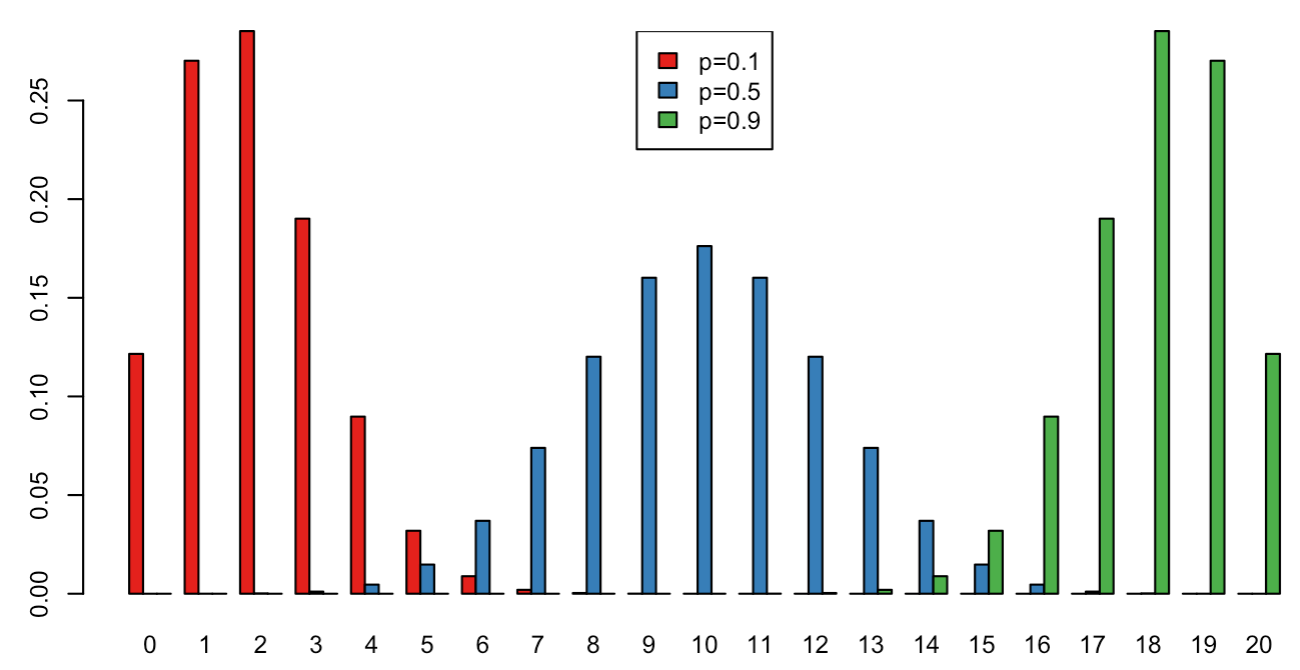
\includegraphics[width=\textwidth]{fig/prob07.png}
    \end{center}

\end{frame}

%%%%%%%%%%%%%%%%%%%%%%%%%%%%%%%%%%%%%%%%%%%%%%%%%%%%%
\begin{frame}
    \frametitle{2. Diskrete Verteilungen: Binomial-Verteilung}

    \begin{itemize}
        \item Beispiel: Polymerase hat eine Fehlerrate von 0.1\%; was ist die Wahrsheinlichkeit, dass eine Sequenz der Länge 1000 3 Fehler enthält?
        \item Wir definieren $X$ als "Anzahl der Fehler in der Sequenz der Länge 1000"
        $$
        P(X=3) = \binom{1000}{3}\,(0.001)^3\,(0.999)^{997} = 0.0612 \sim 6\%
        $$
    \end{itemize}

\end{frame}

%%%%%%%%%%%%%%%%%%%%%%%%%%%%%%%%%%%%%%%%%%%%%%%%%%%%%
\begin{frame}
    \frametitle{Diskrete Verteilungen: 2. Binomial-Verteilung}


    \begin{center}
        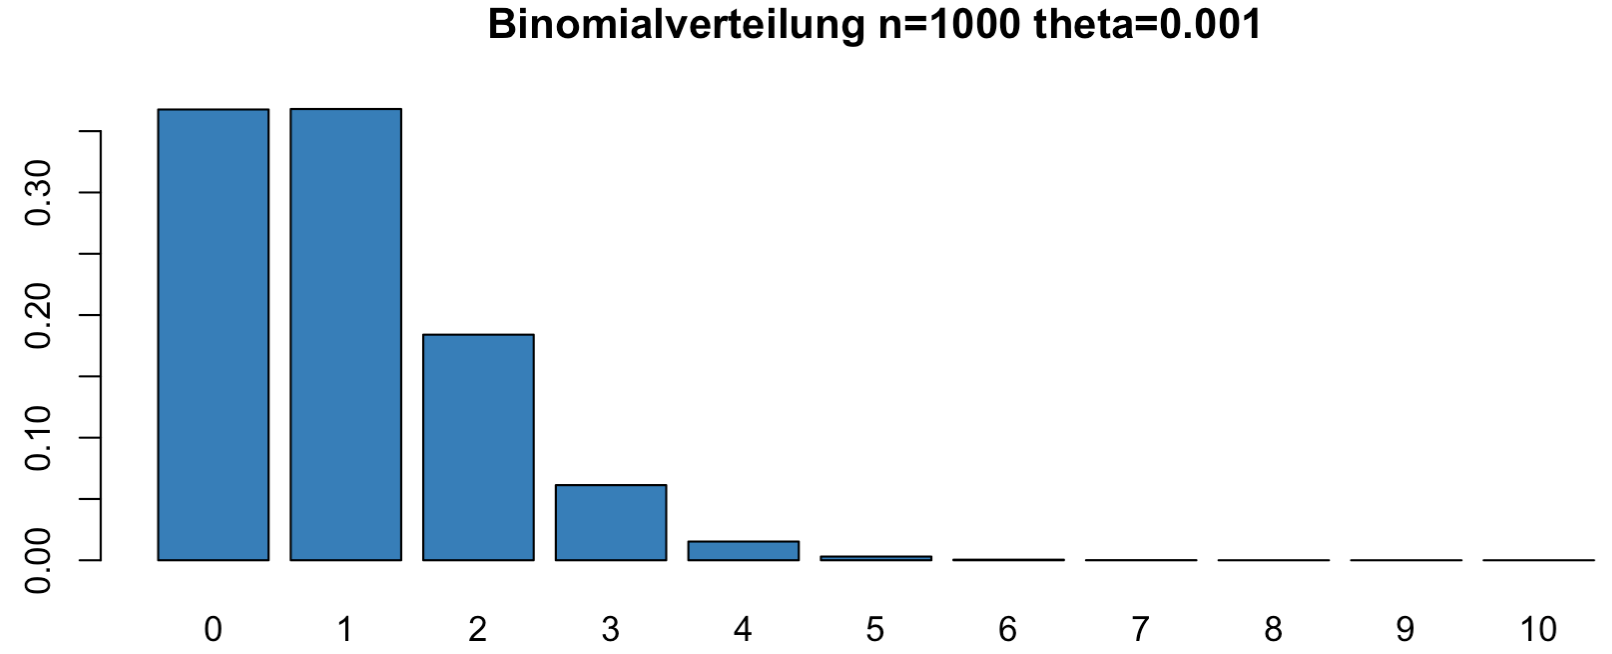
\includegraphics[width=0.8\textwidth]{fig/prob06.png}
    \end{center}

\end{frame}




%%%%%%%%%%%%%%%%%%%%%%%%%%%%%%%%%%%%%%%%%%%%%%%%%%%%%
\begin{frame}
    \frametitle{Diskrete Verteilungen: 3. Poisson-Verteilung}

\begin{itemize}
    \item Die Poisson-Verteilung beschreibt die Anzahl $k$ von erwarteten Ereignissen, wenn die {\bf Rate} $\lambda$ pro Messeinheit bekannt ist
    \item Zufallvariable $X$: Anzahl der beobachteten Ereignisse
    $$
    P(X = k) = \frac{\lambda^k}{k!}\,e^{-\lambda}
    $$
    \item Es gilt:
    $$
    E(X ) = \lambda ~~~~Var(X) = \lambda
    $$
    
\end{itemize}

\end{frame}

%%%%%%%%%%%%%%%%%%%%%%%%%%%%%%%%%%%%%%%%%%%%%%%%%%%%%
\begin{frame}
    \frametitle{Diskrete Verteilungen: 3. Poisson-Verteilung}

\begin{itemize}
\item Beispiel: Es gehen im Durschnitt $\lambda=10$ Anrufen pro Stunde in der Notfallzentrale ein; es wird ein Bonus bezahlt, falls in einer Schicht von 8 Stunden mehr als 100 Anrufen beantwortet werden. Was ist die Wahrscheinlichkeit, dass ein Bonus bezahlt wird?
\item Zufallvariable $X$ = Anzahl der Anrufe in 8 Stunden (Messeinheit = 1 Schicht = 8 Stunden)
\item Rate der Anrufe pro Schicht: $\lambda = 8*10 = 80$
\begin{eqnarray*}
P(X > 100) &=& 1- P(X \le 100) \\
&=& 1- \sum_{k=0}^{100} \frac{\lambda^k}{k!}\,e^{-\lambda} \\
&=& 0.01317 \sim 1.3 \%
\end{eqnarray*}
\end{itemize}
\end{frame}

%%%%%%%%%%%%%%%%%%%%%%%%%%%%%%%%%%%%%%%%%%%%%%%%%%%%%
\begin{frame}
    \frametitle{Stetige Verteilungen: 1.\ Exponential-Verteilung}

    \begin{itemize}
        \item Die Exponential-Verteilung beschreibt {\bf Wartezeiten}
        \item Zufallsvariable $X$ = Wartezeit, bis ein Ereignis vorkommt, wenn die Rate pro Einheit $\lambda$ ist
        \item Wahrscheinlichkeitsdichte:
        $$
f(x) = \lambda\,e^{-\lambda x} ~~~(x \ge 0)~~~~f(x) = 0 ~~~(x<0)
        $$
        \item Es gilt
        $$
        E(X) = \frac{1}{\lambda}~~~~Var(X) = \frac{1}{\lambda^2}
        $$
    \end{itemize}
    

\end{frame}

%%%%%%%%%%%%%%%%%%%%%%%%%%%%%%%%%%%%%%%%%%%%%%%%%%%%%
\begin{frame}
    \frametitle{Stetige Verteilungen: 1.\ Exponential-Verteilung}

    \begin{itemize}
        \item Beispiel: im Durschnitt wartet ein Kunde 20 Minuten in der Warteschleife einer Kundenhotline; was ist die Wahrscheinlichkeit, dass ich schon nach 5 Minuten drankomme?
        \item Zufallsvariable $X$= Wartezeit in Minuten; Rate der Antworten pro Minute: $\lambda = 1/20 = 0.05$
        \item Wir suchen $P(X\le 5)$:
        \begin{eqnarray*}
        P(X \le 5) &=& \int_{-\infty}^5 \lambda\,e^{-\lambda x}\,dx \\
        &=& \int_{0}^5 \lambda\,e^{-\lambda x}\,dx~~~~\text{da $f(x)=0$ für $x<0$} \\
        &=& [-e^{-\lambda x}]_0^5 \\
        &=& 1-e^{-0.05*5} = 0.22 \sim 22 \%
        \end{eqnarray*}
    \end{itemize}
    

\end{frame}

%%%%%%%%%%%%%%%%%%%%%%%%%%%%%%%%%%%%%%%%%%%%%%%%%%%%%
\begin{frame}
    \frametitle{Stetige Verteilungen: 1.\ Exponential-Verteilung}


    \begin{center}
        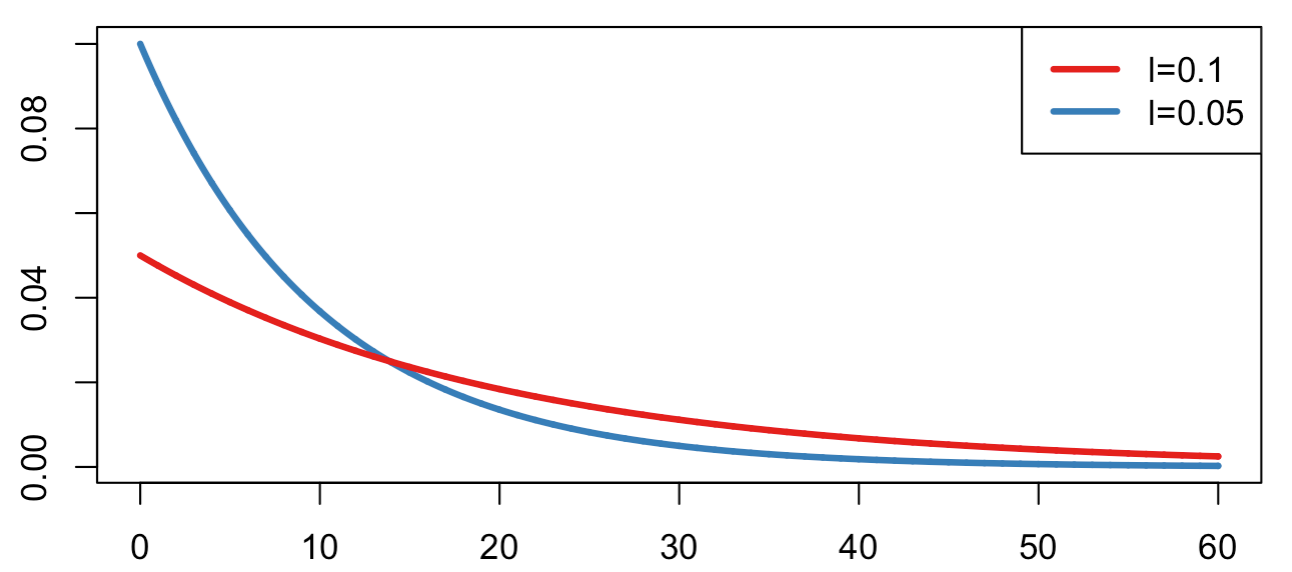
\includegraphics[width=0.8\textwidth]{fig/prob08.png}
    \end{center}

\end{frame}

%%%%%%%%%%%%%%%%%%%%%%%%%%%%%%%%%%%%%%%%%%%%%%%%%%%%%
\begin{frame}
    \frametitle{Stetige Verteilungen: 2.\ Normal-Verteilung}


    \begin{itemize}
        \item Normal-Verteilung (oder Gauss-Verteilung)
        \item Wahrscheinlichkeitsdichte:
        $$
        f(x) = \frac{1}{\sqrt{2\pi\sigma^2}}\,e^{-\frac{(x-\mu)^2}{\sigma^2}}
        $$
        \item Es gilt:
        $$
        E(X) = \mu ~~~~ Var(X) = \sigma^2
        $$
        \item Schreibweise: $X \sim \mathcal{N}(\mu;\sigma^2)$
        \item Standardnormalverteilung: $X \sim \mathcal{N}(0;1)$ ~~$f(x) = \frac{1}{\sqrt{2\pi}}\,e^{-x^2}$
    \end{itemize}

\end{frame}

%%%%%%%%%%%%%%%%%%%%%%%%%%%%%%%%%%%%%%%%%%%%%%%%%%%%%
\begin{frame}
    \frametitle{Normal-Verteilung}

    \begin{center}
        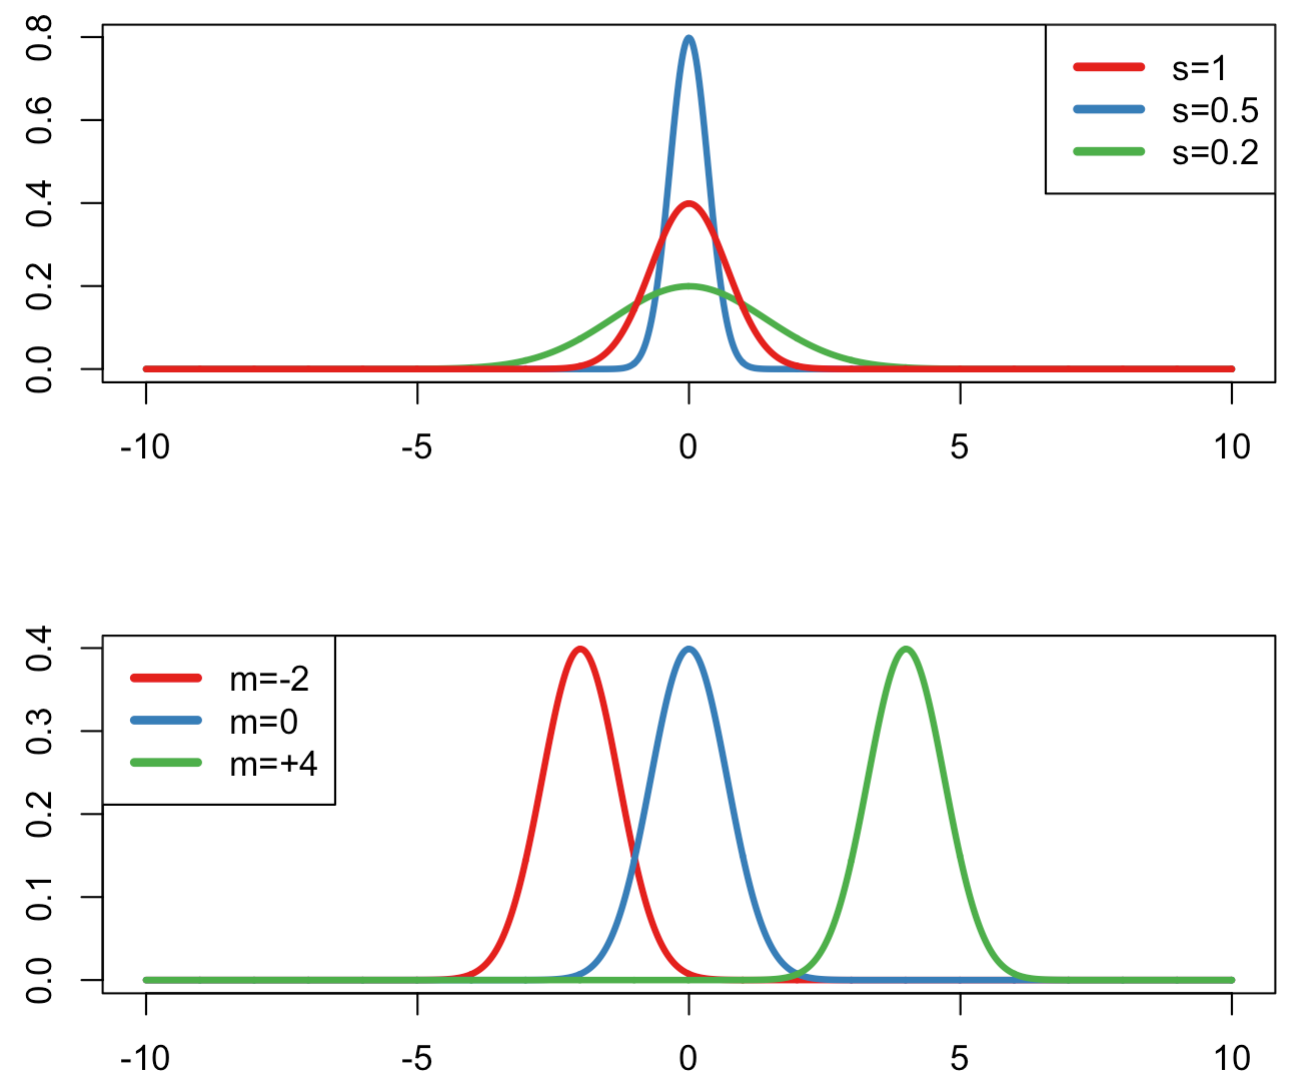
\includegraphics[width=.9\textwidth]{fig/prob10.png}
    \end{center}

\end{frame}


%%%%%%%%%%%%%%%%%%%%%%%%%%%%%%%%%%%%%%%%%%%%%%%%%%%%%
\begin{frame}
    \frametitle{Abschlussfragen}

    \begin{enumerate}
        \item Zeigen Sie, dass der Erwartungswert der Exponential-Verteilung $E(X) = 1/\lambda$ ist.
        \item Zeigen Sie, dass bei der Binomial-Verteilung die Bedingung $\sum_k P(X=k)=1$ erfüllt ist! Benutzen Sie dazu, dass $(a+b)^n = \sum_{k=0}^n \binom{n}{k}a^kb^{n-k}$
        \item Wie groß ist die Wahrscheinlichkeit, dass es unter 100 Personen mindestens eine gibt, die am 10. März Geburtstag hat?
        \item Bestimmen Sie erwartete Anzahl $\lambda$ von Leuten, die in einer Gruppe von 100 am 10. März Geburtstag haben; Bestimmen Sie anhand der Poisson Verteilung $P_{\lambda}(X\ge 1)$ und vergleichen Sie mit der ersten Wahrscheinlichkeit.
        
    \end{enumerate}
    
\end{frame}